\chapter{Methods}
\label{cha:methods}
This chapter contains the methods used for extending the existing hash based digital signature systems in this work.

\section{T5 Hashing}
Dodis et al.~\cite{T5_paper} propose a method called $T5$ for hashing five inputs with three hash compression calls. The $5n$-to-$n$ compression function $T5$ (with $n$ being the hash digest length) is constructed out of $2n$-to-$n$ compression functions $h_1, h_2, h_3$:

\begin{equation}
\label{eq:t5_basic}
T_5(m_1, m_2, m_3, m_4, m_5) = h_3(h_1(m_1,m_2) \oplus m_5, h_2(m_3,m_4) \oplus m_5) \oplus m_5
\end{equation}
It is proven by Dodis et al.~\cite{T5_paper} that the $T5$ construction matches Stam’s bound~\cite{stams_bound2008}, providing $\tilde{\mathcal{O}}(q^2/2^n)$ collision security and $\mathcal{O}(q^3/2^{2n}+nq/2^n)$, $q \leq 2^{n/2}$ preimage security. It provides birthday security $\mathcal{O}(2^{n/2})$ (see also Section~\ref{sec:omit_coll_res}) for hashing 5 inputs using three $2n$-to-$n$ compression calls, instead of only 4 inputs (in prior constructions). For the full proof of collision resistance and preimage resistance of $T5$, see Section~4.1 and Section~4.2 in~\cite{T5_paper}. % what is q not sure
Therefore, $T5$ is improving the Merkle-D\aa mgard construction (with the initialization vector counted as message block) and Merkle trees by processing a fifth message block with the same number of compression function calls and basically the same level of collision security. 
For this work, the construction of $T5$ in combination with Merkle trees is of interest.  

\subsection{T5 Block}
\label{sec:t5_block}
In Figure~\ref{img:t5_paper_block_depiction}, the construction of one \textit{T5-Block} out of a Merkle tree with height $d=2$ is shown:

\begin{itemize}
\item The variables  $m_1, m_2$ (respectively $m_3, m_4$) denote the left and right halves of input to compression function $h_1$ (respectively $h_2$).
\item The variable $a$ (respectively $b$) denotes the output of $h_1$ (respectively $h_2$).
\item The variables $c$ and $d$ denote the left and right halves of input to $h_3$.
\item The variable $e$ denotes the output of $h_3$.
\item The variable $f$ denotes the total output of $T5(m_1, m_2, m_3, m_4, m_5)$.
\end{itemize}
Therefore, the calculation of $T_5(m_1, m_2, m_3, m_4, m_5)$ consists of the following steps:
\begin{enumerate}
\item Calculation of the first layer of one $T_5$-Block (corresponds to compressing 4 leaves of a binary Merkle tree), two hash function calls $h_1, h_2$ are necessary:
\begin{align}
a = h_1(m_1, m_2) \\
b = h_2(m_3, m_4)
\end{align}

\item Calculation of the first $T_5$-specific intermediate step, adding $m_5$:
\begin{align}
c = a \oplus m_5 \\
d = b \oplus m_5
\end{align}

\item Calculation of the second layer of one $T_5$-Block (corresponds to compressing 2 nodes of a binary Merkle tree), one hash function calls $h_3$ is necessary:
\begin{align}
e = h_3(c,d)
\end{align}

\item Adding $m_5$ again (the second $T_5$ specific intermediate step) leads to the final result $f$:
\begin{align}
f = e \oplus m_5 = T_5(m_1, m_2, m_3, m_4, m_5)
\end{align}
\end{enumerate}

\begin{figure}
\centering
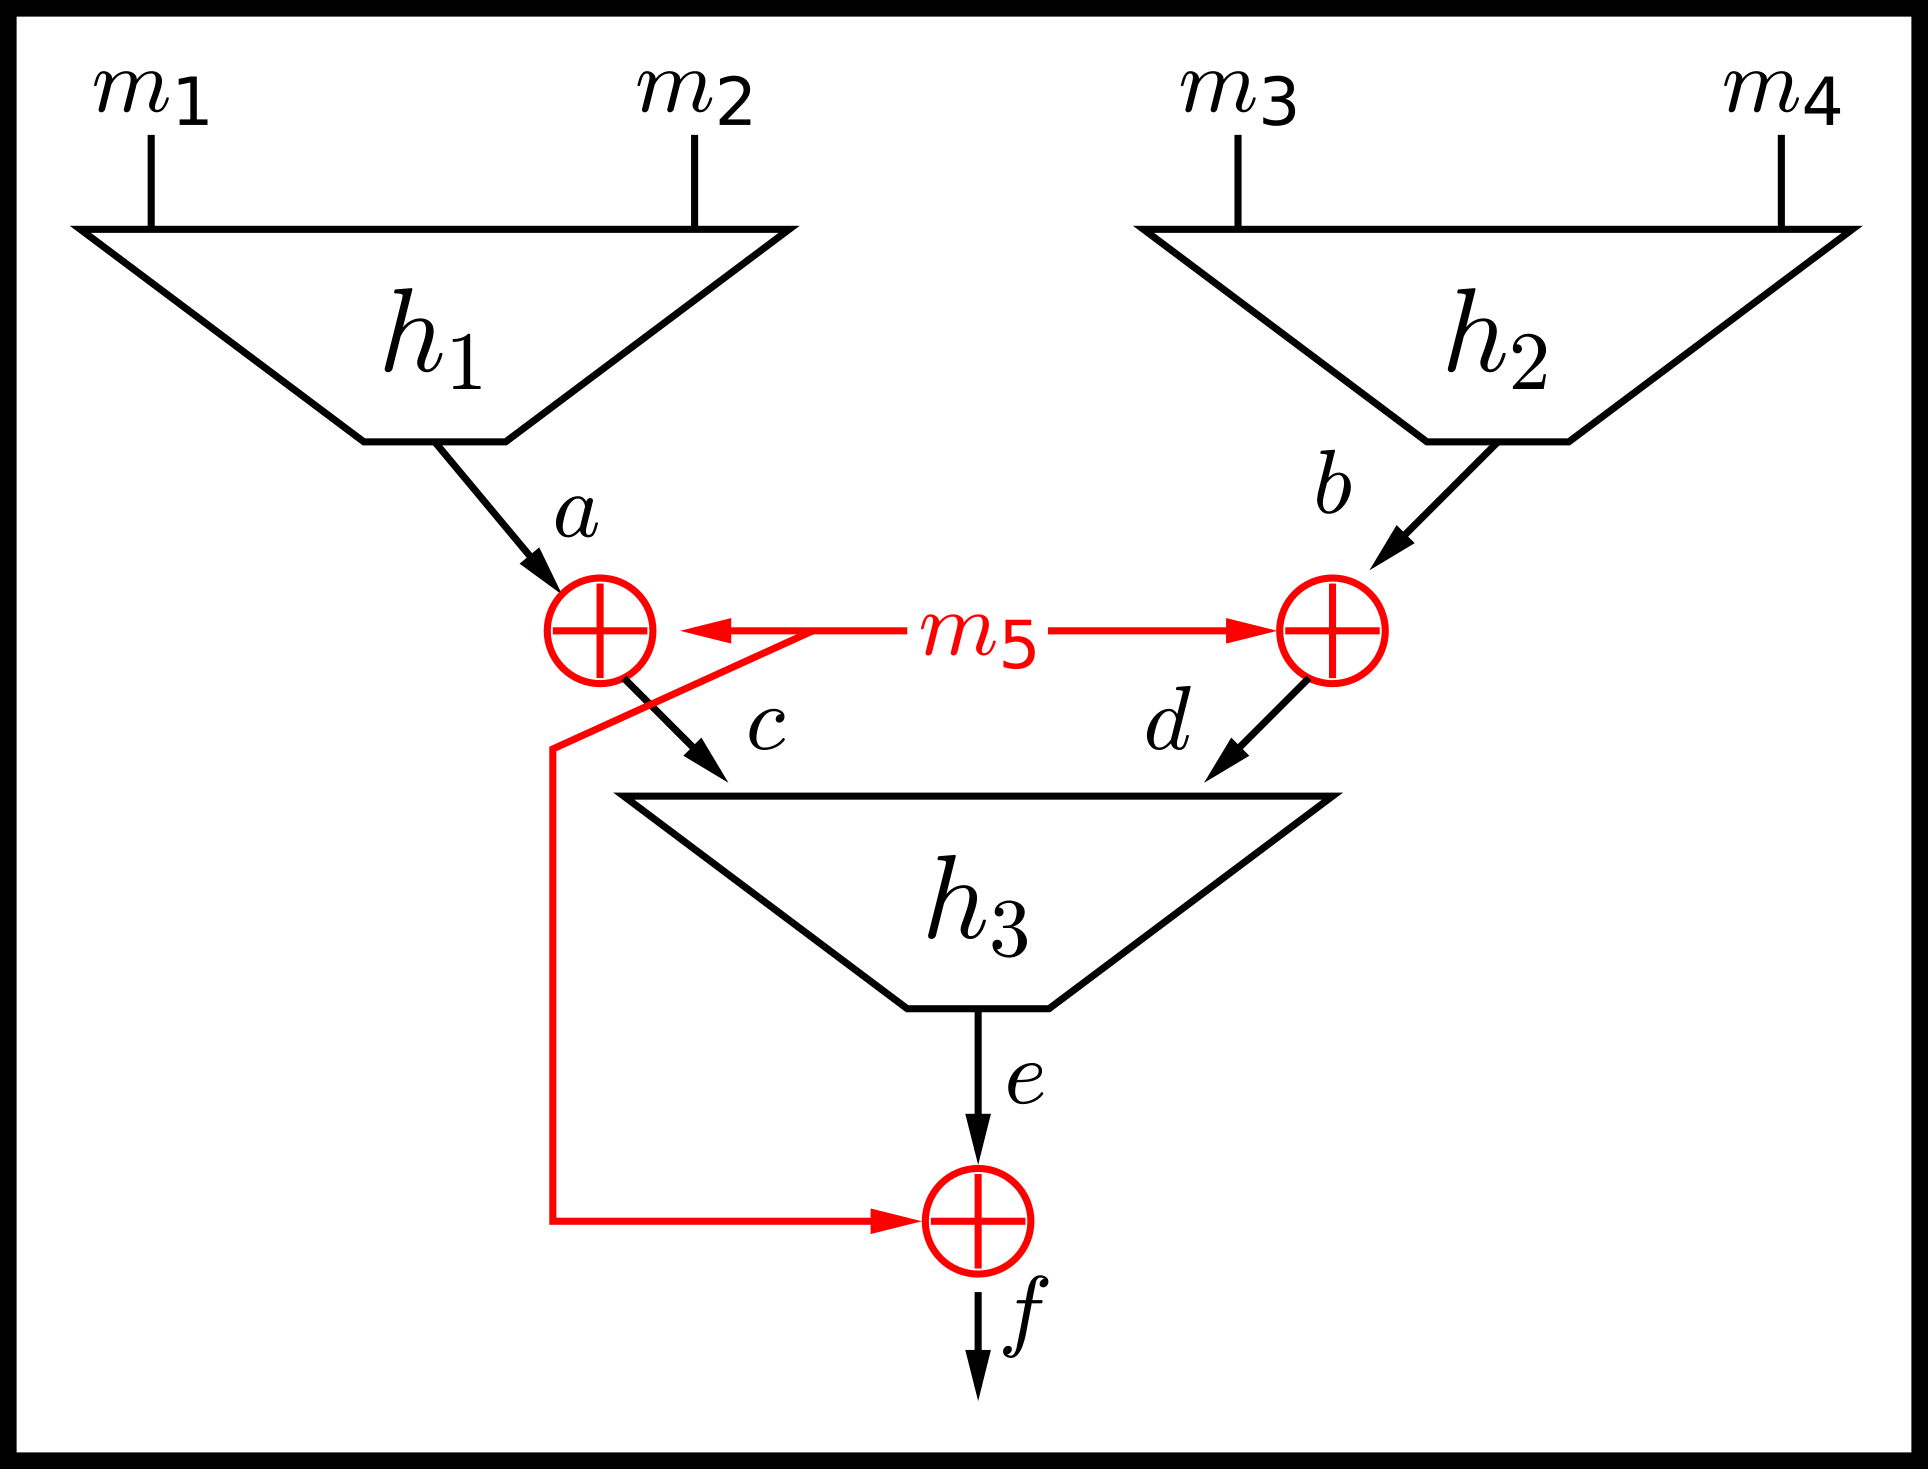
\includegraphics[]{images/Methods/abcd_paperT5_block_depiction.png}
\caption{Modified Merkle tree $T_5(m_1, m_2, m_3, m_4, m_5)$ of height d = 2,   with an extra input $m_5$ for the same 3 hash calls $h_1, h_2, h_3$. In this work, it is referred to as one $T_5$-Block.~\cite{T5_paper}}
\label{img:t5_paper_block_depiction}
\end{figure}

\subsection{T5 Openings}
To calculate the authentication path (see also Section~\ref{sec:mss_sig_gen} ) in one T5-Block, two different approaches \textit{Conservative Opening} and \textit{Aggressive Opening} are shown by Dodis et al.~\cite{T5_paper}. These two versions are depicted in Figure~\ref{img:t5_conserv_aggr_opening}.
The process of calculating an authentication path is here referred to as \textit{opening}. 

\subsubsection{Conservative Opening}
\label{sec:conserv_opening}
Given a node $m_i, i \in \{1,2,3,4\}$, the straightforward way to open the $T_5$-Block is to provide the remaining four nodes $m_{j \neq i}$. This is denoted as Conservative Opening and depicted in Figure~\ref{img:t5_conserv_aggr_opening}: The current node on the path is $m_1$ (colored green), the remaining four nodes (colored red) necessary for the authentication path to open $m_1$ are $m_2, m_3, m_4, m_5$. The functions $h_1, h_2, h_3$ (colored red) have to be calculated. The performance of the Conservative Method is less attractive than of the other methods and even worse than using a standard Merkle Tree: For authenticating one T5-Block, three hash calls and five elements in the authentication path are necessary, see also Table~\ref{table:conserv_opening}. Therefore, this method is not further considered in this work. % reference to authentication method with merkle tree -> #hashcalls, el. in authpath in table

\begin{table}
\centering
\begin{tabular}{l c} 
 \hline\noalign{\smallskip}
 \multicolumn{2}{c}{\textbf{Conservative Opening}} \\
 \hline\noalign{\smallskip}
 \# el. in auth. path & 4 \\
  \# hashcalls verify & 3 \\
 \hline
\end{tabular}
\caption{Performance of calculating the authentication path for one $T_5$-Block with Conservative Opening: The necessary amount of hashcalls and amount of elements in the authentication path are given.}
\label{table:conserv_opening}
\end{table}

\subsubsection{Aggressive Opening}
\label{sec:aggr_opening}
The second version of opening a $T_5$-Block with better performance than Conservative Opening is the Aggressive Opening. The provable security bounds decreases for this method, but the security remains the same under plausible attack scenarios. It is defined as follows: For a given opening node $m_i, i \in \{1,2,3,4,5\}$, the function $open_{aggr}$ returns the authentication path elements for the corresponding $T_5$-Block:

\begin{align}
&open_{aggr}(m_1) = (m_2, m_5, h_2(m_3,m_4) \oplus m_5) = (m_2, m_5, d) \label{eq:aggr_open_m1_example} \\
&open_{aggr}(m_2) = (m_1, m_5, h_2(m_3,m_4) \oplus m_5) = (m_1, m_5, d) \\
&open_{aggr}(m_3) = (m_4, m_5, h_1(m_1, m_2) \oplus m_5) = (m_4, m_5, c) \\ 
&open_{aggr}(m_4) = (m_3, m_5, h_1(m_1, m_2) \oplus m_5) = (m_3, m_5, c) \\ 
&open_{aggr}(m_5) = (m_1, m_2, h_2(m_3, m_4) \oplus m_5) = (m_1, m_2, d) \label{eq:aggr_open_m5_example}
\end{align}
In Figure~\ref{img:t5_conserv_aggr_opening}, Aggressive Opening is depicted as example for opening node $m_1$ (colored green), see Equation~\ref{eq:aggr_open_m1_example}. 
As shown for all opening nodes in Equations~\ref{eq:aggr_open_m1_example}-\ref{eq:aggr_open_m5_example}, with the Aggressive Opening method the authentication path always contains three elements and the verifier needs two hash calls ($h_1$ or $h_2$ respectively and always $h_3$) to calculate the "root" $f$ of one $T_5$-Block, see Table~\ref{table:aggr_opening}.

\begin{table}
\centering
\begin{tabular}{l c} 
 \hline\noalign{\smallskip}
 \multicolumn{2}{c}{\textbf{Aggressive Opening}} \\
 \hline\noalign{\smallskip}
 \# el. in auth. path & 3 \\
 \# hashcalls verify & 2 \\
 \hline
\end{tabular}
\caption{Performance of calculating the authentication path for one $T_5$-Block with Aggressive Opening.}
\label{table:aggr_opening}
\end{table}

\begin{figure}
\centering
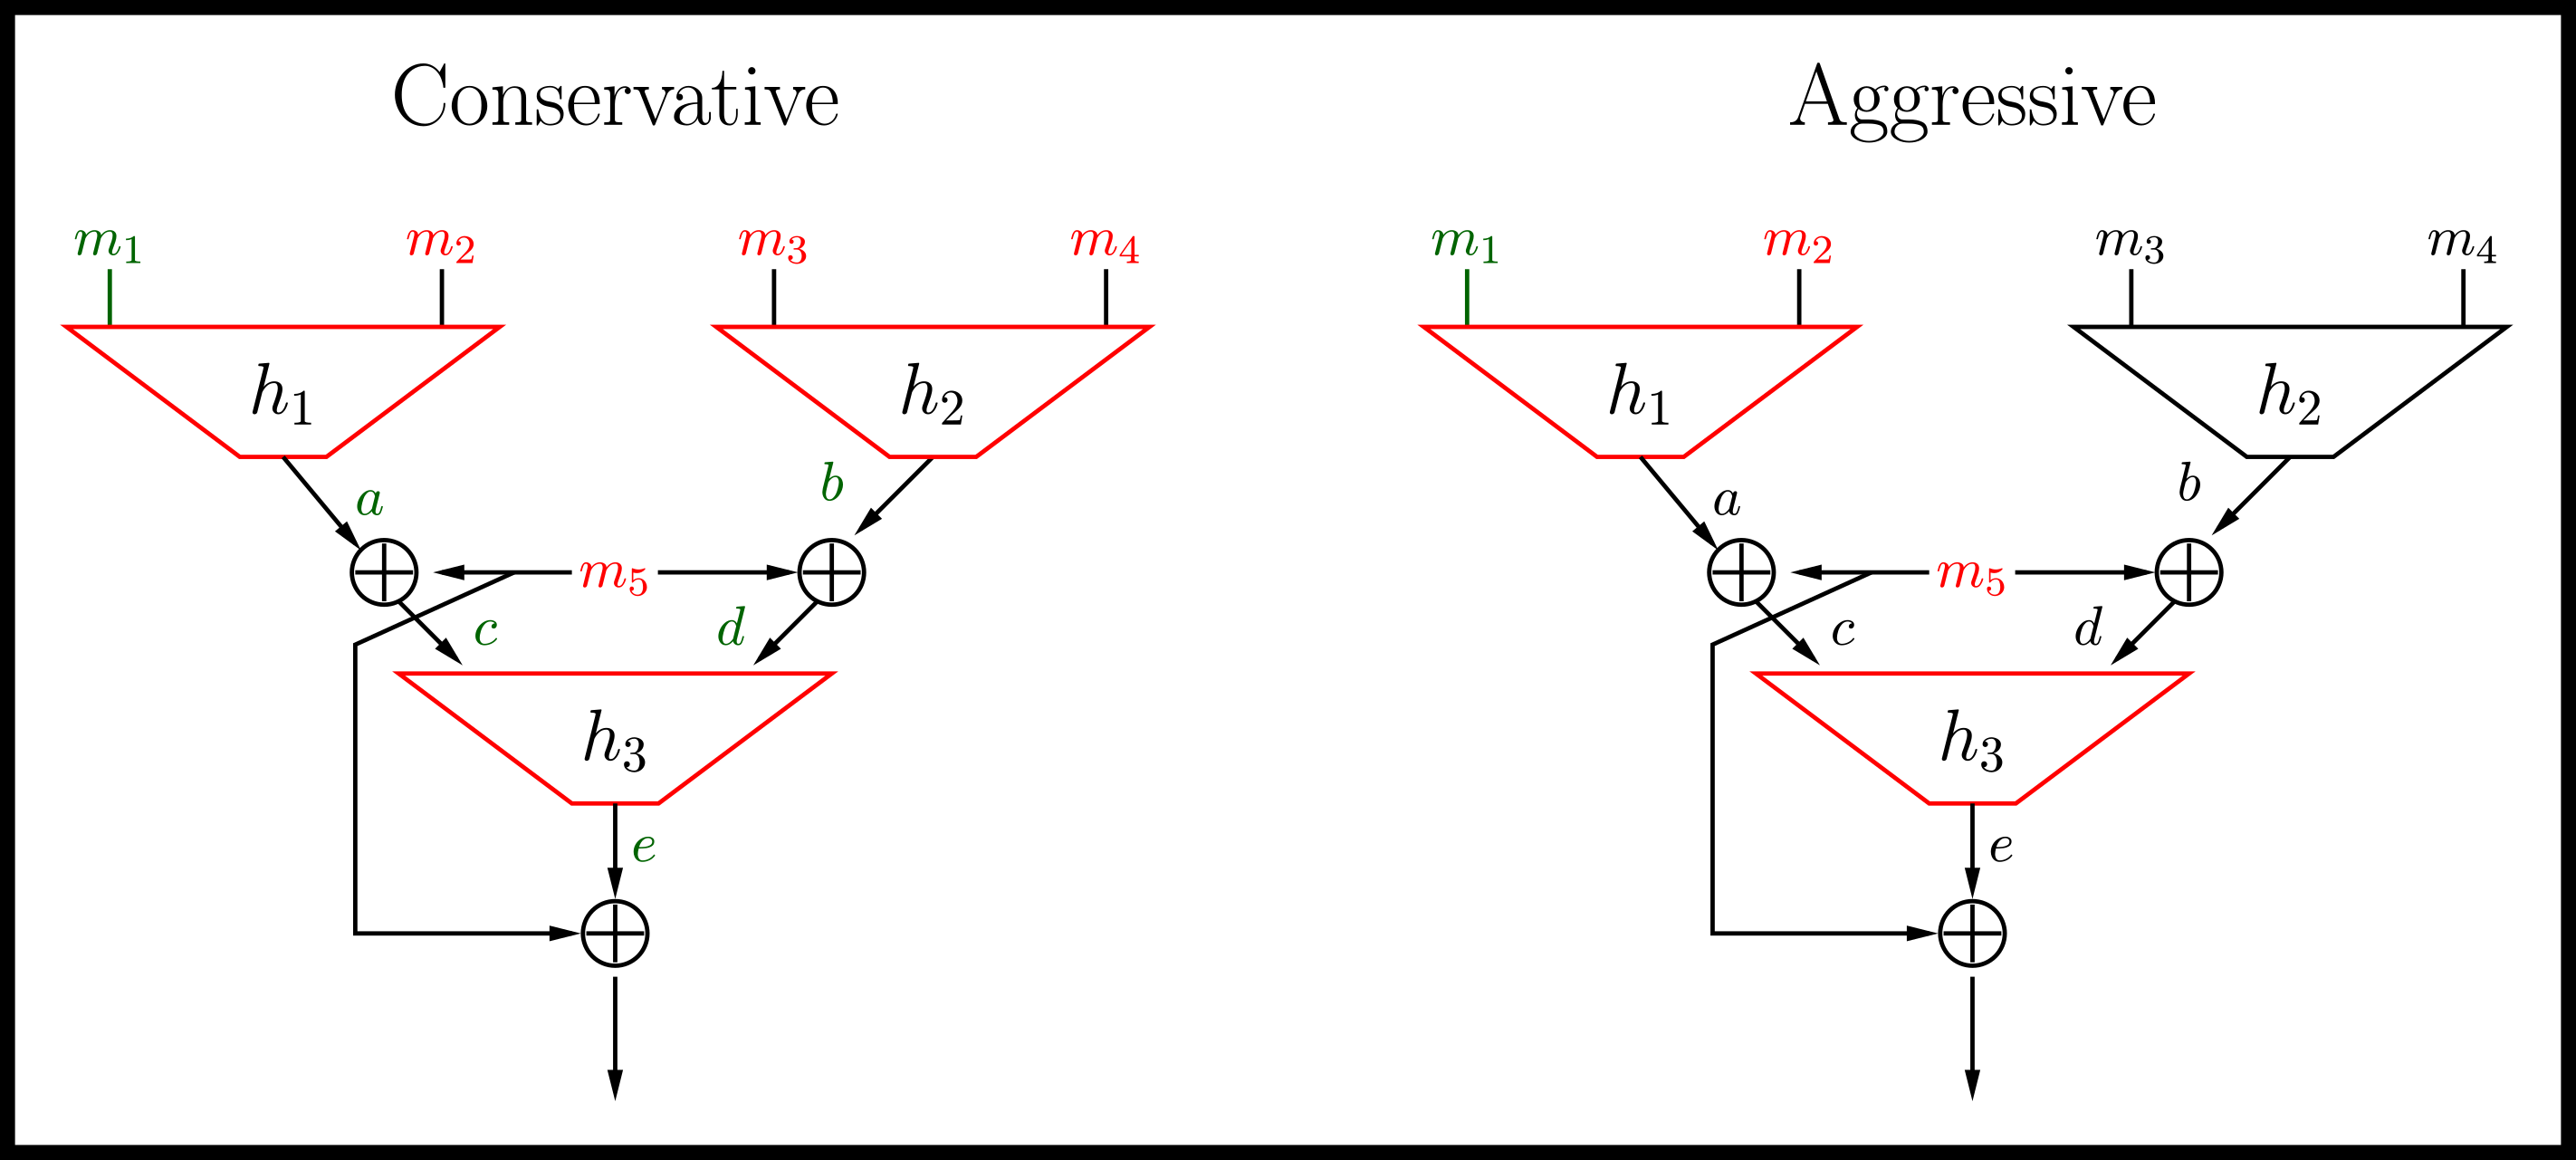
\includegraphics[]{images/Methods/aggr_conserv_opening_T5.png}
\caption{Conservative and Aggressive Opening of one $T_5$-Block. The green variable denotes the opening node, the red nodes are given in the authentication path for this $T_5$-Block. The hash functions denoted in red have to be calculated by the verifier to get the path for this $T_5$-Block.~\cite{T5_paper}}
\label{img:t5_conserv_aggr_opening}
\end{figure}

\subsection{T5 Merkle Tree}
\label{sec:dodis_t5_merkle_tree}
Given the $T_5$-Block construction in Section~\ref{sec:t5_block}, a complete \textit{$T_5$ Merkle Tree}, denoted as \textit{\tftree}, can be built. This is also shown by Dodis et al.~\cite{T5_paper}, see Figure~\ref{img:t5_complete_tree_paper}. Notably, the compression functions $h_1, h_2, h_3$ are the same function, the different indices are used for readability. The performance of the \tftree (including Conservative- and Aggressive Opening variants) in comparison to the standard Merkle Tree is shown in Table~\ref{table:t5_merkletree_dodis_performance}: \textit{Build calls} denote the amount of hash calls necessary for building the whole $T_5$ Merkle Tree, \textit{opening} denotes thee length of the authentication path, \textit{verify} denotes the amount of hash calls needed to build the path (out of the authentication path). \textit{Tree depth} is the amount of layers in the binary Merkle tree compared with the amount of layers in \tftree - this corresponds to the amount of $T_5$ blocks $\times 2$ because one \tfblock corresponds to two Merkle tree layers (see also Figure~\ref{img:t5_paper_block_depiction}).

\begin{table}
\centering
\begin{tabular}{l c c c} 
 \hline\noalign{\smallskip}
 \multicolumn{4}{c}{\textbf{$T_5$ Merkle Tree Performance}} \\
 \hline\noalign{\smallskip}
 & Merkle Tree (standard) & Conserv. Opening &  Aggr. Opening \\
 \hline\noalign{\smallskip}
 build calls$/t$ & 1 & 0.75 & 0.75 \\
 tree depth$/\log_2(t)$ & 1 & 0.86 & 0.86 \\
 verify (hash calls)$/\log_2(t)$ & 1 & 1.29 & 0.86 \\
 opening (length)$/\log_2(t)$ & 1 & 1.72 & 1.29 \\ 
 \hline
\end{tabular}
\caption{Performance of the $T_5$ Merkle Tree with the opening variants Conservative- and Aggressive Opening in comparison to the standard Merkle Tree given by Dodis et al.~\cite{T5_paper}. The variable $t$ denotes the amount of children.}
\label{table:t5_merkletree_dodis_performance}
\end{table}

\begin{figure}
\centering
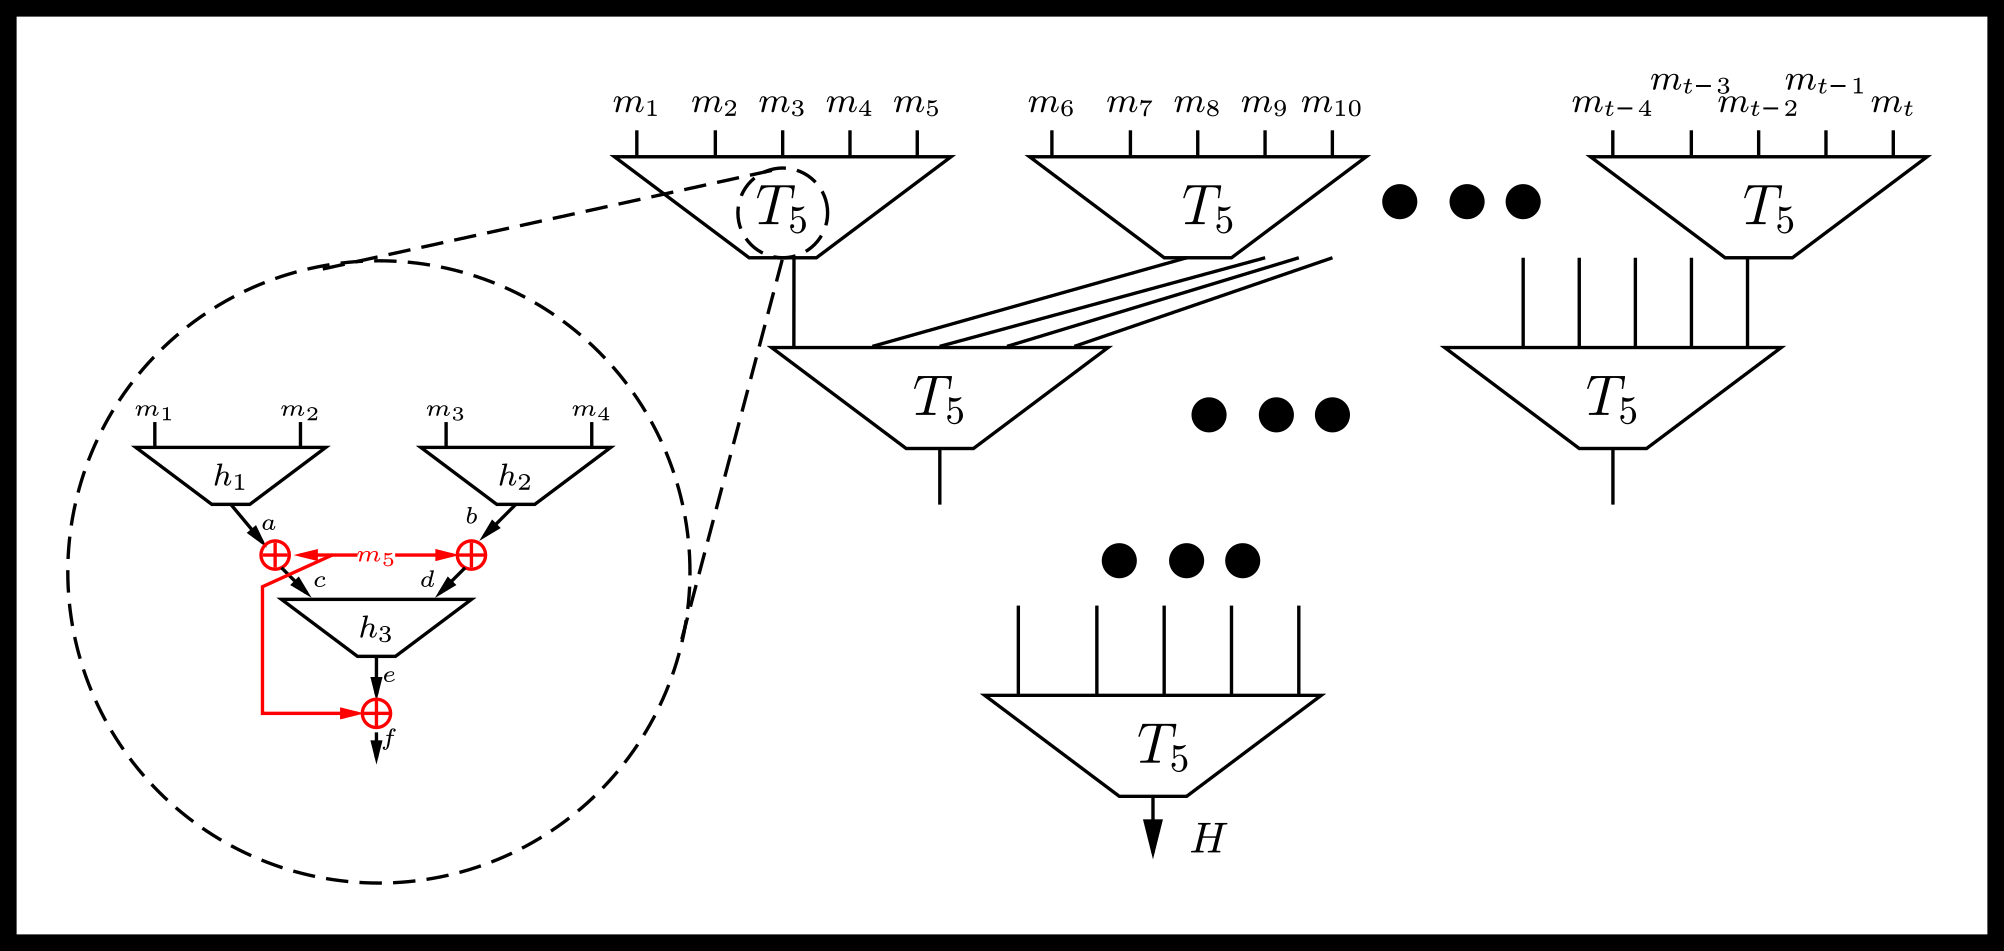
\includegraphics[]{images/Methods/whole_tree_T5_paper.png}
\caption{Construction of a complete $T_5$-Tree consisting of several $T_5$-Blocks~\cite{T5_paper}. The value $H$ denotes the root of the tree.}
\label{img:t5_complete_tree_paper}
\end{figure}

\section{Extended T5 Merkle Tree}
\label{sec:ext_t5_tree} % "my idea"
In this section, the idea of the \tftree is extended by an opening method \textit{More Aggressive Opening}. When implemented in the whole $T_5$~Merkle tree, the tree construction is denoted as \textit{\extree}.
The performance of \extree is compared to \tftree with Aggressive Opening of Dodis et al.~\cite{T5_paper}. There is also a python implementation of \extree as digital signature scheme that contains the steps from key generation to signature verification, see Appendix~\ref{cha:appendix_t5_tree_implementation}.
The parameters used for \extree construction are denoted in Table~\ref{table:t5_ext_parameter}.


\begin{table}
\centering
\begin{tabular}{c l}
 \hline\noalign{\smallskip}
 \multicolumn{2}{c}{\textbf{\extree Parameter}} \\
 symbol & meaning \\
 \hline\noalign{\smallskip} 
 $T$ & height of the tree in $T_5$-Blocks. $T = \log_5(\ell)$ \\
  $\ell$ & amount of leaves. $\ell = 5^T$ \\
 $d$ & height of the tree in actual Merkle nodes. $d = 3T$ \\
 \hline
\end{tabular}
\caption{The parameters of \extree. Notably, one \tfblock contains three Merkle layers, therefore $d=3T$ (see also Figure~\ref{img:t5_paper_block_depiction}).} % explain correlation T, d -> d = 3T really correct? maybe picture of T5Tree+?`
\label{table:t5_ext_parameter}
\end{table}

\subsection{More Aggressive Opening}
\label{sec:more_aggr_opening}
In this work, the new opening method \textit{More Aggressive Opening} is proposed, see Figure~\ref{img:t5_more_aggr_opening}. It has better overall performance than Conservative- and Aggressive Opening (see Section~\ref{sec:aggr_opening} and \ref{sec:conserv_opening}) for the signing and verifying process, see Table~\ref{table:more_aggr_opening}. But notably, the length of the authentication path is \textbf{not} constant.

\subsubsection{Signature Generation: \texorpdfstring{\tfblock}{T5-Block}}
When calculating the authentication path (generating the signature) for one \tfblock, two cases distinguished:

\begin{itemize}
\label{list:case1_case_2}
\item \textbf{Case~1}: The possible opening nodes are $m_i, i \in \{1,2,3,4\}$. For a given opening node $m_i$, the function $open_{aggr+}$ returns the authentication path for the corresponding \tfblock:
\begin{align}
open_{aggr+}(m_1) = (m_2, m_5, h_2(m_3, m_4)) = (m_2, m_5, b) = A_{m_1+} \label{eq:more_aggr_m1_example} \\
open_{aggr+}(m_2) = (m_1, m_5, h_2(m_3, m_4)) = (m_1, m_5, b) = A_{m_2+} \\
open_{aggr+}(m_3) = (m_4, m_5, h_1(m_1, m_2)) = (m_4, m_5, a) = A_{m_3+} \\
open_{aggr+}(m_4) = (m_3, m_5, h_1(m_1, m_2)) = (m_3, m_5, a) = A_{m_4+} \label{eq:more_aggr_m4_example}
\end{align} 
An example of $m_1$ as opening node is depicted on the left side of Figure~\ref{img:t5_more_aggr_opening}: The signer is putting the elements $m_2, m_5, b$ in the authentication path (see Equation~\ref{eq:more_aggr_m1_example}). The verifier needs two hash calls ($h_1, h_3$) to calculate the path to the root $f$.
Therefore, the authentication path has always three elements and the verifier always needs two hash calls to calculate the path to the root of one \tfblock for case~1, see also Table~\ref{table:more_aggr_opening}.

\item \textbf{Case~2}: The opening node is $m_5$. This case is depicted on the right side of Figure~\ref{img:t5_more_aggr_opening}. For $m_5$ as opening node, the function $open_{aggr+}$ returns the authentication path for the corresponding \tfblock:
\begin{equation}
\label{eq:more_aggr_opening_m5_example}
open_{aggr+}(m_5) = (h_1(m_1, m_2), h_2(m_3, m_4)) = (a, b) = A_{m_5+}
\end{equation}
An example of $m_5$ as opening node is depicted on the right side of Figure~\ref{img:t5_more_aggr_opening}: The signer is putting the elements $a, b$ in the authentication path (see Equation~\ref{eq:more_aggr_opening_m5_example}). The verifier needs one hash call $h_3$ to calculate the path to the root $f$.
Therefore, the authentication path has always two elements and the verifier always needs one hash call to calculate the path to the root for one \tfblock for case~2, see also Table~\ref{table:more_aggr_opening}.
\end{itemize} 

\begin{figure}
\centering
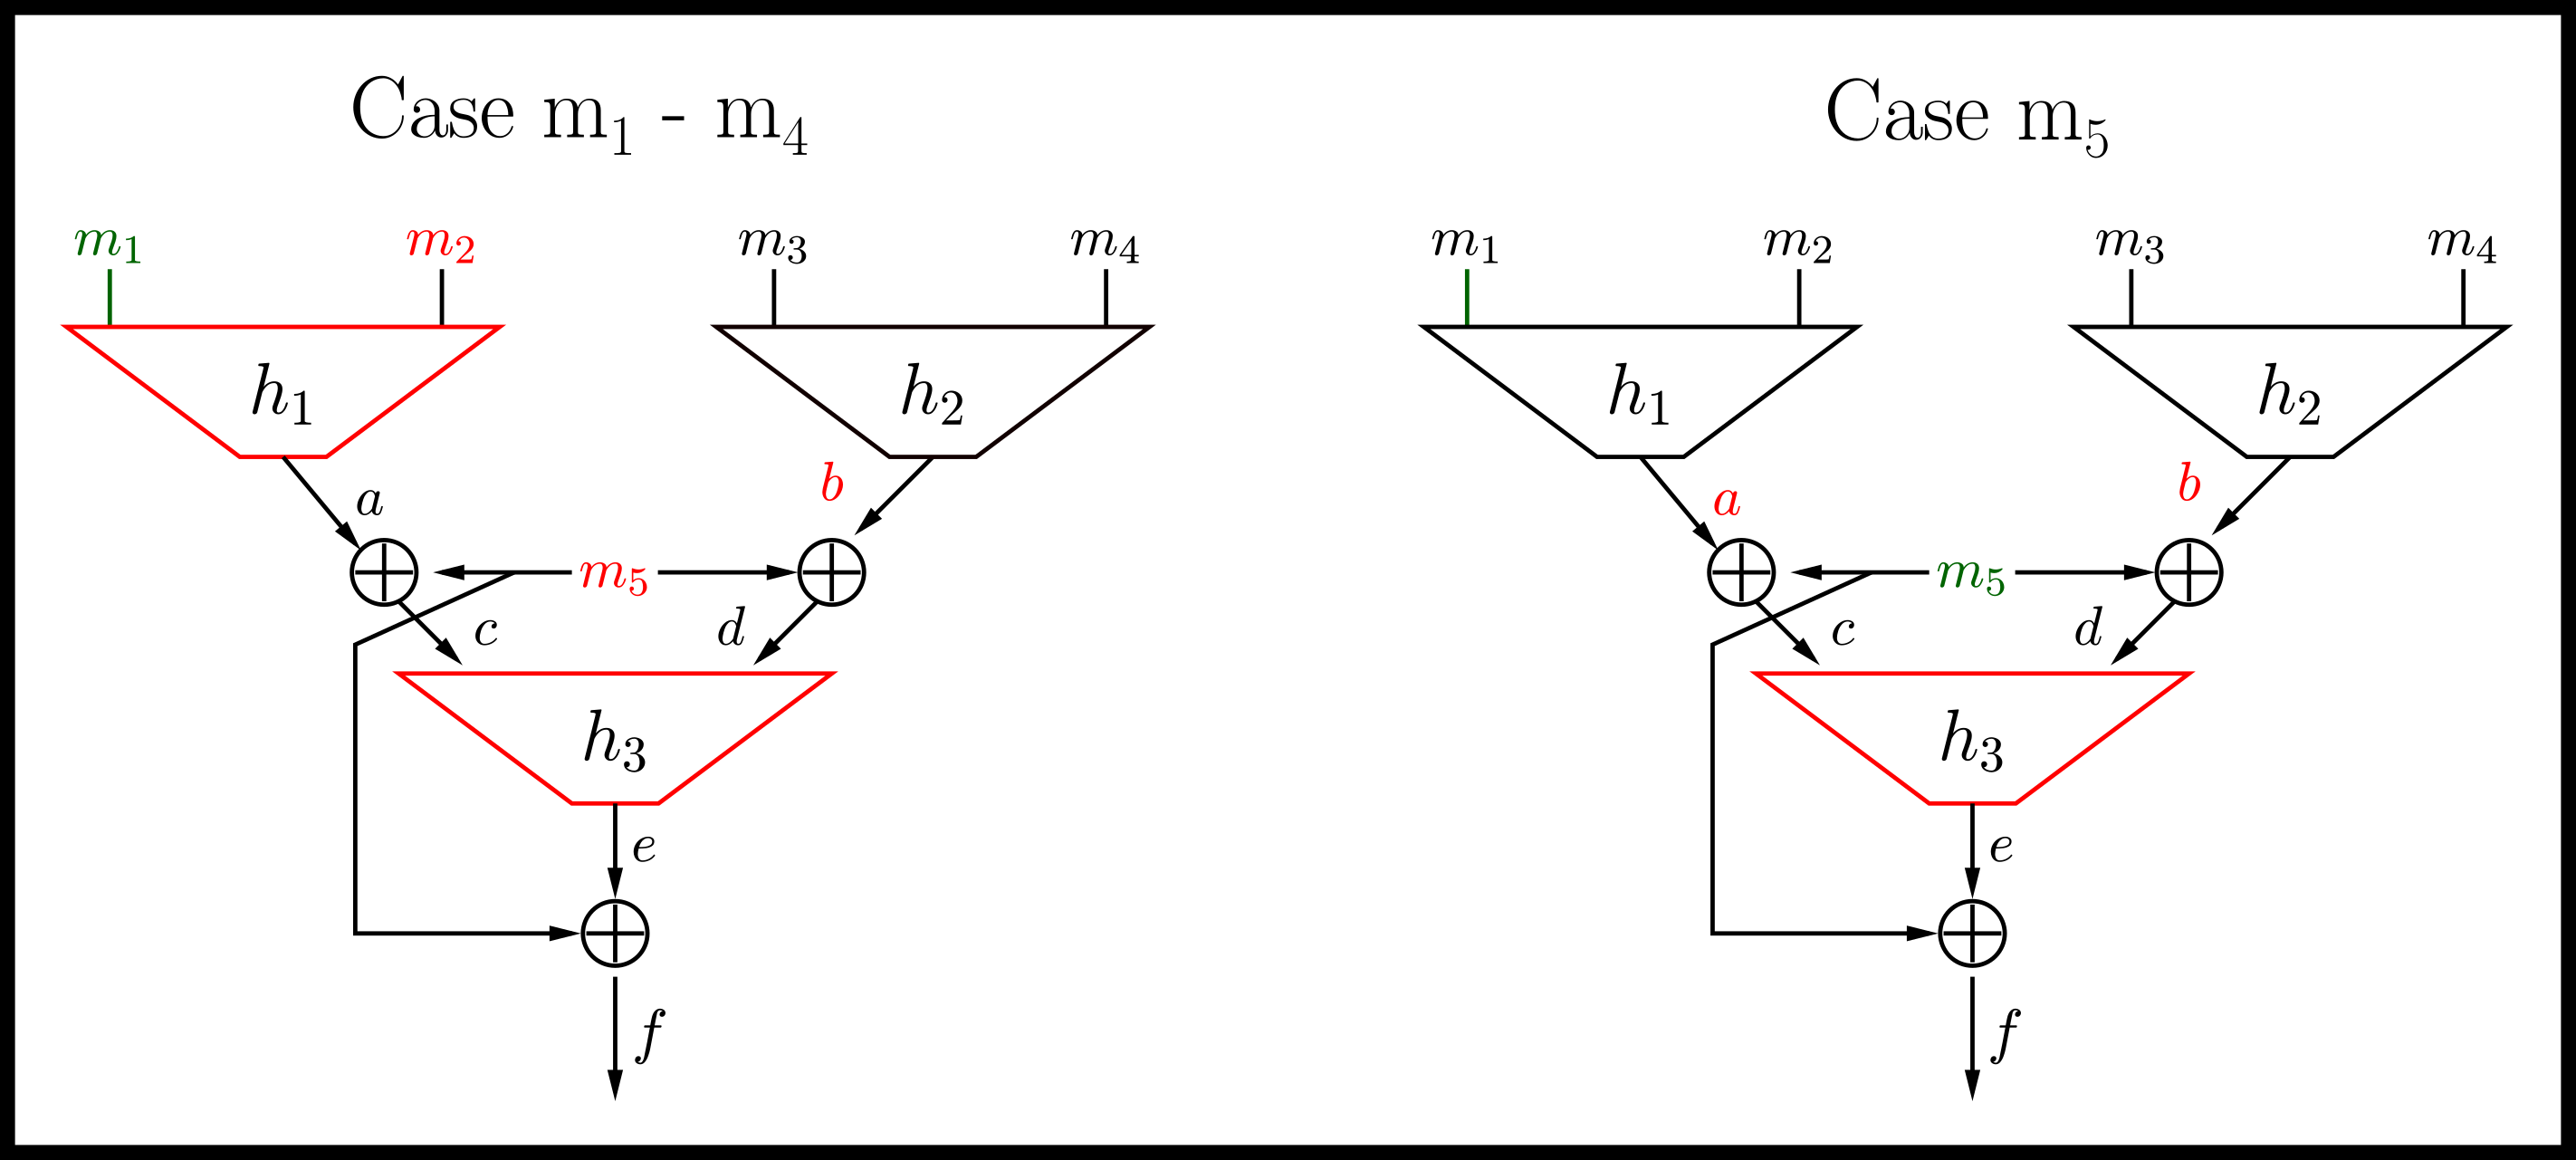
\includegraphics[]{images/Methods/more_aggr_opening.png}
\caption{More Aggressive Opening for one \tfblock, with case differentiation. The green variable denotes the opening node, the red nodes are given in the authentication path the respective \tfblock. The hash functions denoted in red have to be calculated by the verifier to get the path for this \tfblock.}
\label{img:t5_more_aggr_opening}
\end{figure}

\begin{table}
\centering
\begin{tabular}{l c c} 
 \hline\noalign{\smallskip}
 \multicolumn{3}{c}{\textbf{More Aggressive Opening}} \\
 \hline\noalign{\smallskip}
 & case 1: $m_i, i \in \{1,2,3,4\}$ & case 2: $m_5$ \\
 \# el. in auth. path & 3 & 2 \\
 \# hashcalls verify & 2 & 1 \\
 \hline
\end{tabular}
\caption{Performance of calculating the authentication path and amount of elements in the authentication path for More Aggressive Opening. The case~1 with $m_i, i \in \{1,2,3,4\}$ as possible opening/path nodes and case~2 with $m_5$ as opening/path node are shown.}
\label{table:more_aggr_opening}
\end{table}

\subsubsection{Signature Verification: \texorpdfstring{\tfblock}{T5-Block}}
When calculating the path (verifying the signature) for one \tfblock, the same two cases as for signature generation are distinguished (see Equation~\ref{eq:more_aggr_m1_example}-\ref{eq:more_aggr_m4_example} and Equation~\ref{eq:more_aggr_opening_m5_example} respectively). For an explanatory depiction of the two cases, see Figure~\ref{img:t5_more_aggr_opening}.

\begin{itemize}
\item \textbf{Case~1}: The possible leaves of the \tfblock, for which a path to the root $f$ will be calculated by the verifier, are $m_i, i \in \{1,2,3,4\}$. For leaf $m_i$ and the corresponding authentication path $A_{m_i+}$ (given by the signer, see Equation~\ref{eq:more_aggr_m1_example}-\ref{eq:more_aggr_m4_example}), the function $path(m_i,A_{m_i+})$ returns the root $f$ for the corresponding \tfblock:

\begin{align}
&path(m_1, A_{m_1+}) = path(m_1, (m_2, m_5, b)) = h_3(h_1(m_1, m_2) \oplus m_5, b \oplus m_5) \oplus m_5 = f \label{eq:more_aggr_path_m1}\\
&path(m_2, A_{m_2+}) = path(m_2, (m_1, m_5, b)) = h_3(h_1(m_1, m_2) \oplus m_5, b \oplus m_5) \oplus m_5 = f\\
&path(m_3, A_{m_3+}) = path(m_3, (m_4, m_5, a)) = h_3(a \oplus m_5, h_2(m_3, m_4) \oplus m_5) \oplus m_5 = f \\
&path(m_4, A_{m_4+}) = path(m_4, (m_3, m_5, a)) = h_3(a \oplus m_5, h_2(m_3, m_4) \oplus m_5) \oplus m_5 = f \label{eq:more_aggr_path_m4}
\end{align}

\item \textbf{Case~2}: The path $f$ needs to be calculated for $m_5$ as given "leaf" of the \tfblock. Given $m_5$ and the corresponding authentication path $A_{m_5+}$ (given by the signer, see Equation~\ref{eq:more_aggr_opening_m5_example}) is calculated by $path(m_5, A_{m_5+})$:
\begin{equation}
\label{eq:more_aggr_path_m5}
path(m_5, A_{m_5+}) =  path(m_5, (a,b)) = h_3(a \oplus m_5, b \oplus m_5) \oplus m_5 = f
\end{equation}
\end{itemize}

The process of tree generation, signing and verifying using Aggressive Opening in the \extree is shown in the following section. 


\subsection{\texorpdfstring{\extree}{Ext. T5-Tree} Generation}
The \extree Generation works like tree generation for the \tftree, see Section~\ref{sec:dodis_t5_merkle_tree}, Section~\ref{cha:mss_keygen} and Figure~\ref{img:t5_complete_tree_paper}. The implementation of the \extree construction in Python is shown in Appendix~\ref{cha:appendix_t5_tree_implementation}.
% maybe pseudocode but too complex -> just read appendix
% 
The performance equations for building an \extree are derived as follows (see also Table~\ref{table:t5_ext_parameter}). the total amount of \tfblocks in one \extree is:
\begin{equation}
\text{\#\tfblocks} = \sum_{i=0}^{T-1} 5^i
\end{equation} 
For one \tfblock, three hash calls are necessary (see Section~\ref{sec:t5_block}). Therefore, the total amount of hash calls for building \extree based on $T$ is:\\
\begin{equation}
\text{\# hash calls tree gen. (depending on $T$)} = 3 \cdot \sum_{i=0}^{T-1} 5^i
\end{equation}
To get the hash calls for tree generation based on the leaves $\ell$, $T$ is substituted by $\log_5(\ell)$.
\begin{equation}
\text{\# hash calls tree gen. (depending on $\ell$)}=3 \cdot \sum_{i=0}^{\log_5(\ell)-1} 5^i = 3 \cdot \sum_{i=0}^{\frac{\log(\ell)}{\log(5)}-1} 5^i = \frac{3}{4} (\ell-1)
\end{equation}

\subsection{\texorpdfstring{\extree}{Ext. T5-Tree} Signature Generation}
The signature generation for \extree works as follows: After calculating the complete \extree, the signer first calculates the $T_5$-Path (see also line~17, \mintinline{python}{def calc_t5_path}~($\cdots$) in Appendix~\ref{cha:appendix_t5_tree_implementation}).
Now, the signer calculates the authentication path out of the $T_5$-Path (see also line~167, \mintinline{python}{def calc_auth_path}~($\cdots$) in Appendix~\ref{cha:appendix_t5_tree_implementation} and Section~\ref{sec:mss_sig_gen}).

For this version of the \extree, it is assumed the signer saves the whole tree  after key generation. Therefore, no additional hash calls are necessary for generating the authentication path. % maybe insert #hashcalls for winternitz ots generation
As \extree uses More Aggressive Opening, the length of the authentication path differs on the case, see Section~\ref{sec:more_aggr_opening}.
For \textbf{case~1}, there are always three elements in the authentication path for one \tfblock, see Equation~\ref{eq:more_aggr_m1_example}-\ref{eq:more_aggr_m4_example} and Table~\ref{table:more_aggr_opening}.
For \textbf{case~2}, there are always two elements in the authentication path, see Equation~\ref{eq:more_aggr_opening_m5_example}. For of all signatures used in one \extree, the average of \textbf{case~1} is $\frac{4}{5}$ , whereas the average \textbf{case~2} is $\frac{1}{5}$.
Therefore, the average amount of elements in the authentication path is calculated as follows:
\begin{equation}
\label{eq:more_aggr_len_authpath}
\text{\# elements auth.path (average)} = 3 \cdot \frac{4}{5} + 2 \cdot \frac{1}{5} = 2.8
\end{equation}

\subsection{\texorpdfstring{\extree}{Ext. T5-Tree} Signature Verification}
After receiving the authentication path by the signer, the verifier calculates the path through the \extree to its root (see also line~28, \mintinline{python}{def calc_path_verifier}~($\cdots$) in Appendix~\ref{cha:appendix_t5_tree_implementation}). The verifier compares the calculated root with the public key of the signer, if they match, the signature is valid (see Section~\ref{sec:mss_sign_verif}).

With the More Aggressive opening variant used in the \extree, calculating the path for \textbf{case~1} needs two hash calls (see Equation~\ref{eq:more_aggr_path_m1}-\ref{eq:more_aggr_path_m4}) and calculating it for \textbf{case~2} needs one hash call (see Equation~\ref{eq:more_aggr_path_m5}). The average of each case over of all signature verifications (for one \extree), is $\frac{4}{5}$ for\ \textbf{case~1} and $\frac{1}{5}$ for \textbf{case~2}. Therefore, the average amount of hash calls necessary for calculating the root $f$ of the \extree is calculated as follows:

\begin{equation}
\text{\# hash calls path calculation} = \frac{4}{5} \cdot 2 + \frac{1}{5} = 1.8
\end{equation}

